
\mainsection{5}{Advanced optimization techniques}{15/05/2020}
\section{Difficulties in optimization }
2 Questions:
\textbullet universal approximation: Existence of a NN for each task\\
Will you find it?\\
\textbullet Why was the conventional NN not successful? \\
\putfigure{1.0}{1}{0.4}{Images/1DVisualizaitonOptimization}{1D Visualization Gradient Descent} 
%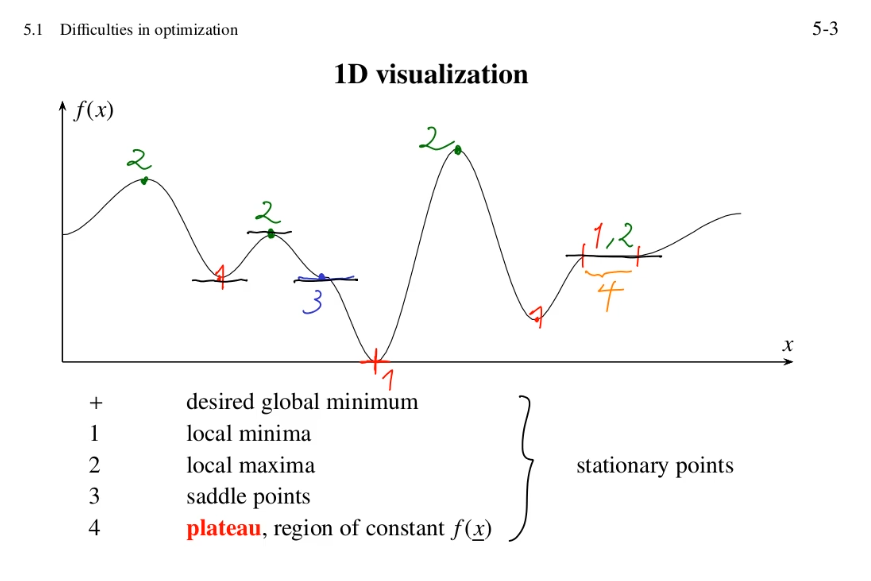
\includegraphics[width = \linewidth]{Images/1DVisualizaitonOptimization.png}\\
\putfigure{1.0}{1}{0.4}{Images/2DConturLines}{2D Contour lines} 
% 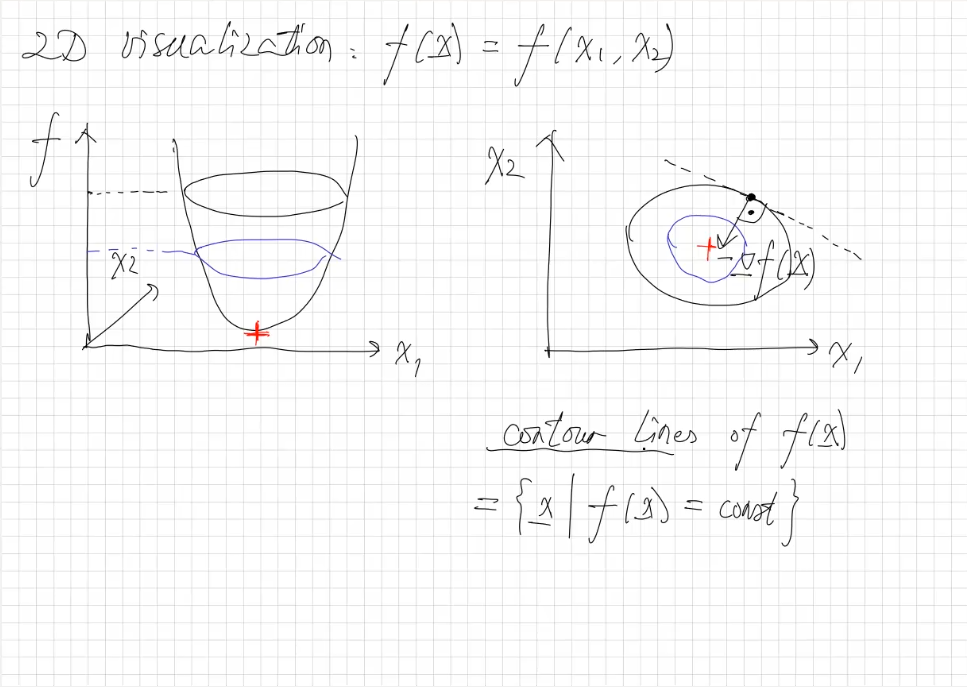
\includegraphics[width = \linewidth]{Images/2DConturLines.png}\\
\putfigure{1.0}{1}{0.4}{Images/IllConditioning}{Ill conditioning} 
%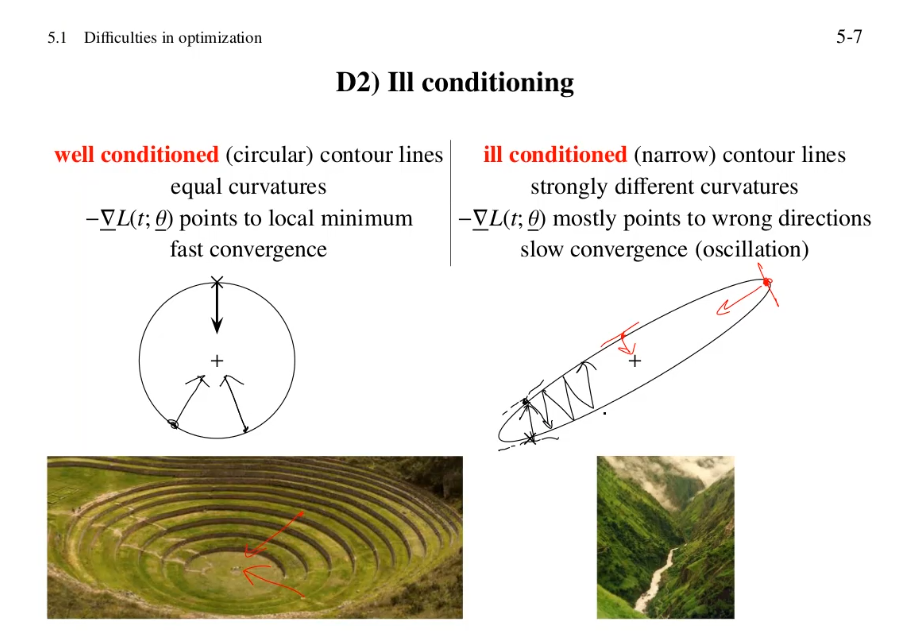
\includegraphics[width = \linewidth]{Images/IllConditioning.png}\\
\textbf{D3) Saddlepoint and plateau}
$  \underline{\nabla} L = \underline{0}  $ no update of $  \underline{x}^t $ because correction term is 0\\
in practice: $  \underline{\nabla} L \approx \underline{0} \rightarrow  $ very slow convergence\\
\putfigure{1.0}{1}{0.4}{Images/SensitiveChoiceStepsize}{Sensitive Choice for step size} 
%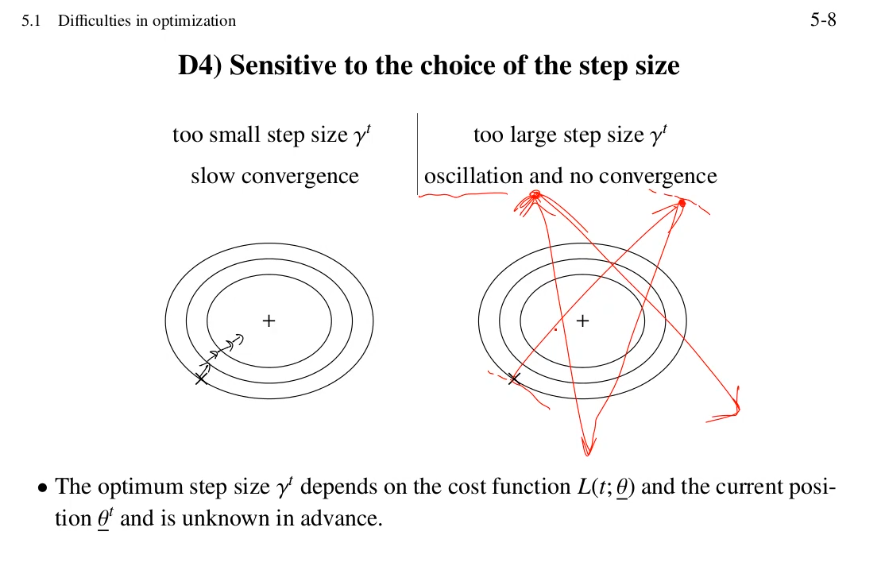
\includegraphics[width = \linewidth]{Images/SensitiveChoiceStepsize.png}\\
 \textbf{Vanishing Gradient:}\\
 Backpropagation of the error vector \\
 $  \Theta = \dfrac{\partial L (\underline{\theta}}{\partial \underline{a}_L} \in \Re^{1 \times M_L} $ in 4.7:\\
 $  \underline{\delta}_1^T = \underline{ \delta}_L ^T \cdot \underline{\underline{j}}_{\underline{a}_L} (\underline{a}_{L-1}),.., \underline{\underline{J}}_{\underline{a}_2} (\underline{a}_1) $, L Layers\\
 $ \underline{\underline{J}}_{\underline{a}_{L+1}} (\underline{a}_L) = \underline{\underline{J}}_{\underline{a}_{L+1}} (\underline{x}_l) \cdot \underline{\underline{J}}_{\underline{x}_L} (\underline{a}_L) = \underline{\underline{W}}_{l+1} \cdot diag( \phi'_{L} (\underline{a}_L))   $\\
 if $  || \underline{\underline{J}}_{\underline{a}_{L+1}} (\underline{a}_L) || < 1, \forall l $ matrix norm , then $  || \underline{\delta}_L || \rightarrow 0  $ \\
 vanishing gradient $\rightarrow$ no update of $  \underline{\theta}^T $ stop learning. 
 With the multiplication of a lot of terms smaller than 1 the gradient turns to a very small number close to zero \\
\textbullet if $  || \underline{\underline{J}}_{\underline{a}_{l+1}} (\underline{a}_l) || > 1, \forall l, $  then $ ||\underline{\delta}_l || \rightarrow \infty $\\
exploding gradient $\rightarrow$ divergence \\
no problem for shallow NN's because only small number of layers \\
bo problem for deep NN's because of large number of layers \\
\textbullet vanishing gradient less serious for the last layers $ (l \uparrow) $ \\
\textbullet more serious for first layers $ (l \downarrow) $ 
\subsection{E5.1: sigmoid vs. ReLU}
\textbf{a) sigmoid or tanh:} \\
$ \phi (a) = \sigma(a) = \dfrac{1}{1+ e^{-a}} \in (0,1) $ \\
if $ |a| >> 1: \phi'(a) \approx 0 $ due to saturation (shape of function )\\
$\rightarrow$ sigmoid bad for DNN die to vanishing gradient \\
\textbf{b) ReLU}\\
$  \phi (a) = max (0,a) $\\
$  \phi' (a) = \left\lbrace \begin{array}{lc}
1 & a > 0 \\
0 & a < 0
\end{array} \right. = u(a) $ \\
$\rightarrow$ ReLu less serious for vanishing gradient
\section{Momentum method}
an improvement of SGD \\
\textbullet change from $  \underline{\theta}^t $ to $ \underline{\theta} ^{t+1}: \Delta \underline{\theta}^t =\beta \cdot \Delta \underline{\theta}^{t-1}  \underbrace{  - \gamma^t \underline{\nabla}   L(t; \underline{\theta}) |_{\underline{\theta} = \underline{\theta}^t}}_{\text{gradient part}} $\\
\textbullet update: $  \underline{\theta}^{t+1} = \underline{\theta}^{t} + \delta \underline{\theta}^t $ \\
$  0 \leq \beta \leq 1 :  $ \textbf{momentum factor}\\
$  \beta =0 $ : SGD \\
$  \beta > 0  $ : recursive smoothing of $  \Delta \underline{\theta}^t $  \\
\textbf{Effect of the momentum: } \\
\textbullet reduce noise in stochastic gradient (D1) \\
\textbullet reduce oscillation and accelerate the convergence of the gradient method for ill conditioned contour lines(D2) 
\subsection{Nesterov Momentum}
a variant of momentum method \\
$  \Delta \underline{\theta} ^{t} =\beta \Delta \underline{\theta}^{t-1} +  \underbrace{(- \gamma^t \underline{ \nabla} L(t; \underline{\theta})|_{ \underline{\theta} = \underline{\theta}^t + \beta \Delta \underline{\theta}^t)}}_{\text{lookahead gradient at the predicted position } \underline{\theta}^{t-1} + \beta \Delta \underline{\theta}} $ 
\section{5.3 Learning rate schedule}
How to choose the step size /learning rate $  \gamma^t $?\\
Many possible schedules \\
\textbf{S1 constant learning rate:}\\
$ \gamma^t = \gamma = const., \forall t $\\
But difficulty D4: \\
\textbullet $  \gamma $ too small: slow convergence \\
\textbullet $  \gamma $ too large: no convergence / oscillation around local minimum\\
$\rightarrow$ Need a trade-off between \\
\textbullet fast convergence at the beginning: $  \gamma \uparrow $ (large step size) \\
\textbullet less oscillation afterwards : $  \gamma \downarrow $ reduce stepsize with growing number of iterations: \textbf{learning rate decay} \\
\textbf{Weakness:}\\
\textbullet manual choice of $ \gamma_0, t_0 , c $\\
\textbullet same schedule for all parameters in $ \underline{\theta} $ \\
\textbf{Adaptive schedules:}
\textbullet different schedules for different parameters in $  \underline{\theta} $\\
\textbullet $ \gamma^t  $ calculated dynamically depending on $ \underline{\theta}^t $ \\
Slide 5-16 Adam very popular \\
